\documentclass[letterpaper,11pt]{article}
\usepackage[utf8]{inputenc}
\pagestyle{empty}
\usepackage[leqno]{amsmath}
\usepackage{amssymb,mathtools}
%\usepackage[activeacute,spanish]{babel}
\usepackage{ucs}
%\usepackage[applemac]{inputenc}
%\usepackage[T1]{fontenc} tipo de letra
\usepackage[scaled]{berasans}
\usepackage{amssymb}
\usepackage[section]{placeins}
\usepackage{color,soul}
\usepackage{amsmath,latexsym,amsthm,mathrsfs}
\usepackage{setspace}
\usepackage{psfrag}
\usepackage{graphicx}
\usepackage{enumerate}
\usepackage{float}
\usepackage{preview}
\usepackage{standalone}
\usepackage{multirow,array}
\usepackage{caption}
\usepackage{subcaption}
%%%%TIKS
\usepackage{pgf,tikz}
\usepackage{tkz-graph}
\usetikzlibrary{arrows,%
	petri,%
	topaths}%
%\usepackage{tkz-berge}
%\usepackage[position=top]{subfig}
%\usepackage[spanish]{babel}
%\documentclass[tikz,border=10pt]{standalone}
\usetikzlibrary{positioning}
\tikzset{main node/.style={circle,fill=white!20,draw,minimum size=1cm,inner sep=0pt},
}
\newcommand{\R}{\mathbb{R}}
\newcommand{\Q}{\mathbb{Q}}
\newcommand{\F}{\mathcal{F}}
\newcommand{\C}{\mathcal{C}}
\newcommand{\FF}{\mathscr{F}}
\newcommand{\CC}{\mathscr{C}}
\newcommand{\DD}{\mathscr{D}}
\newcommand{\D}{\mathcal{D}}
\newcommand{\T}{\mathcal{T}}
\newcommand{\A}{\mathcal{A}}
\newcommand{\B}{\mathcal{B}}
\newcommand{\PP}{\mathbb{P}}
\newcommand{\EE}{\mathbb{E}}
\newcommand{\VV}{\mathbb{V}ar}
\newcommand{\naturales}{n\in\mathbb{N}}
\newcommand{\N}{\mathbb{N}}
\newcommand{\NN}{\mathbb{N}}
\newcommand{\p}{\partial}
\newcommand{\ssi}{\Leftrightarrow}
\newcommand{\imp}{\Rightarrow}
\newcommand{\Ssi}{\Longleftrightarrow}
\newcommand{\Imp}{\Longrightarrow}
\newcommand{\ind}{\mathds{1}}
%\renewcommand*\familydefault{\sfdefault}
%\usepackage[charter]{mathdesign}
\usepackage{dsfont} 
\usepackage{multicol}
\usepackage{anysize}
%\usepackage[nocomma]{optidef}

\usepackage[left=2cm,top=2cm,right=2cm, bottom=2cm]{geometry}
\usepackage{fancyhdr}
\pagestyle{fancy}
%\fancypagestyle{plain}%{%
\fancyhf{}
\lhead{\footnotesize\itshape\bfseries\rightmark}
\rhead{\footnotesize\itshape\bfseries\leftmark}
%\pagestyle{plain}
\thispagestyle{empty}


\begin{document}
\title{SCIO}
\maketitle

\section*{Data preparation}
The raw data consists on two dataframes, SCIO and DXA. The former contains the results of all the SCIO measurements, plus additional feature information for each measurement. The latter contains the results from the DXA measurements. 

\begin{table}[h]
	\centering
	\begin{tabular}{l|l|lll}
		Feature Name       & Description                & Values                     &  &  \\ \cline{1-3}
		folio              & Woman ID                   & Numeric                    &  &  \\
		mama               & Breast identifier          & right, left, left2         &  &  \\
		ubicacion          & Location                   & 3pm, 6pm, 9pm, 12pm &  &  \\
		bmi                & Body Mass Index            & Numeric                   &  &  \\
		fitzpatrick\_color & Skin color classification  & II, III, IV, V             &  &  \\
		copa\_sosten       & Bra size                   & A, B, C, D                 &  &  \\
		edad               & Age                        & Numeric                    &  &  \\
		spectrum 0-330     & SCIO spectrum measurements & Numeric                    &  & 
	\end{tabular}
\caption{SCIO Table column information}
\end{table}

\begin{table}[h]
	\centering
	\begin{tabular}{l|l|lll}
		Feature Name       & Description                & Values                     &  &  \\ \cline{1-3}
		folio              & Woman ID                   & Numeric                    &  &  \\
		mama               & Breast identifier          & right, left, left2         &  &  \\
		dxa\_density          & Breast density measured using DXA                   & Numeric &  &  
	\end{tabular}
	\caption{DXA Table column information}
\end{table}

After merging both tables, we have
\begin{itemize}
	\item 197 folios.
	\item 3 breast per folio.
	\item 5 locations per breast.
	\item 3 spectrum measurements per location
\end{itemize}

\section*{Variability within left breast measurements}
We examine now how much does the variability of the SCIO measurements can be attributed to differences in the breast locations, and how much is due the imprecisions of the instrument. The following histogram illustrates the percentage variation between the two measurements of the left breast for each folio, and the percentage variation of a folio with respect to the average.


\begin{figure}[ht!]
	\centering
	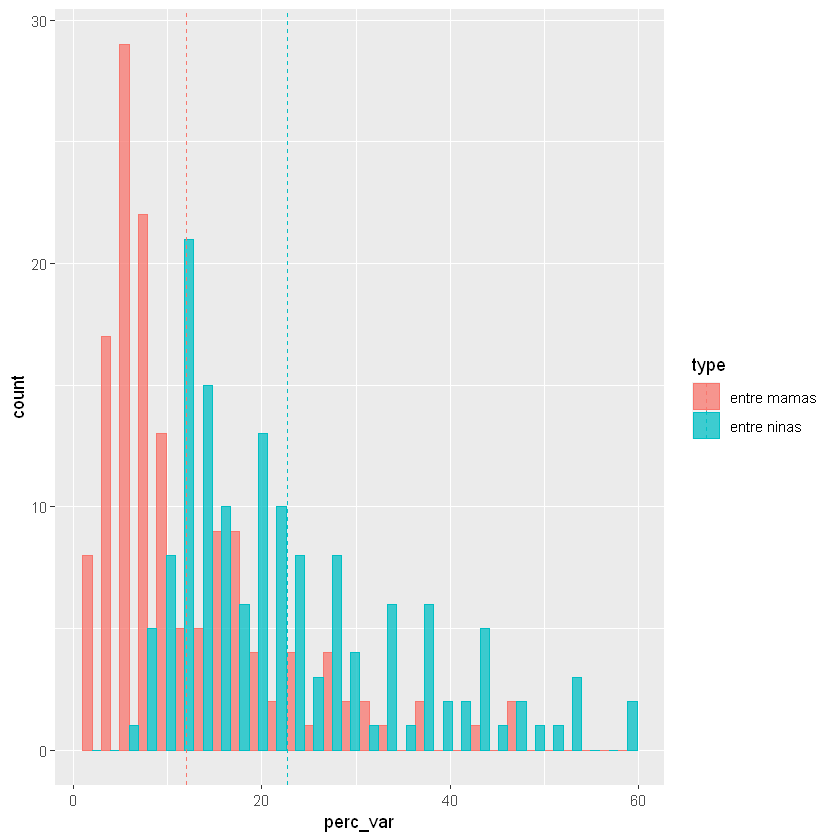
\includegraphics[trim={0 0cm 0cm 0}, clip, scale=0.55]{figures/variability_histogram.png}
	\caption{Variability of measurements across women and across breasts for the same woman.} 
	\label{fig:variability}
\end{figure}

Around 30\% of folios have a left breast variation that is indistinguishable from the variation between folios.  We decided to remove those entries from our analysis and predictions.

\section*{Distribution Analysis}
We begin by analyzing the distribution of DXA density values in Figure \ref{fig:dxa}. The blue dashed lines correspond to the 25\%, 50\% and 75\% quantiles.
\begin{figure}[!htb]
	\centering
	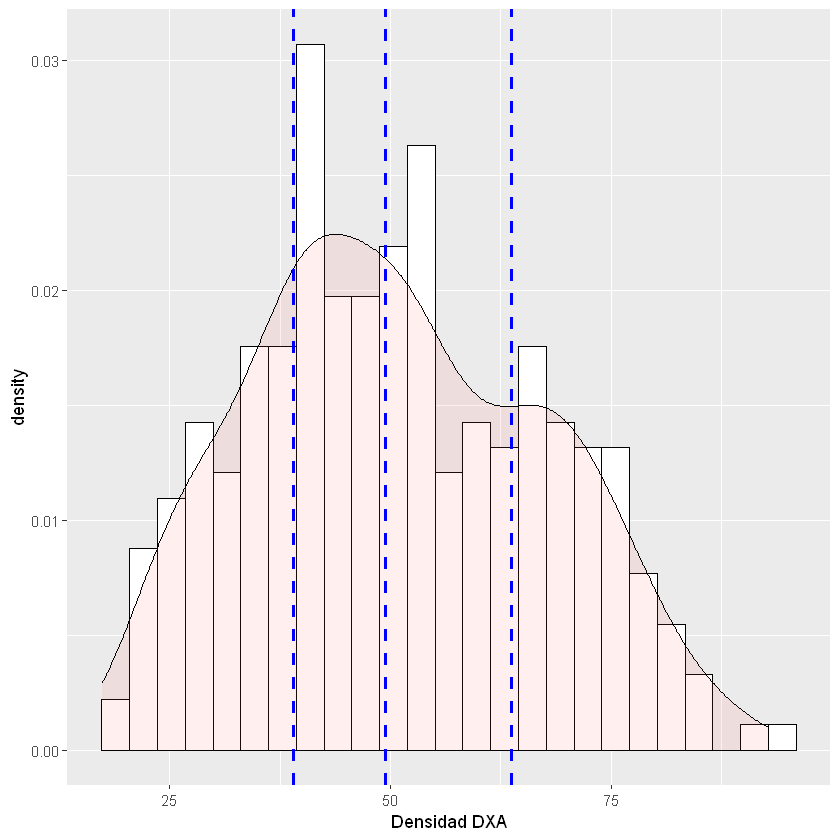
\includegraphics[trim={0 0cm 0cm 0}, clip, scale=0.55]{figures/distribution_dxa.png}
	\caption{Distribution of DXA density.} 
	\label{fig:dxa}
\end{figure}

Then we analyze the distribution of spectrum values per breast separated by BMI. As a way to illustrate differences in density, we color code the entries with high DXA density in red (75\% quantile) and low DXA density in blue. We perform the same analysis for Copa Sosten and Fitzpatrick Color, and we also consider the mean values within each category.
\begin{figure}[!htb]
	\centering
	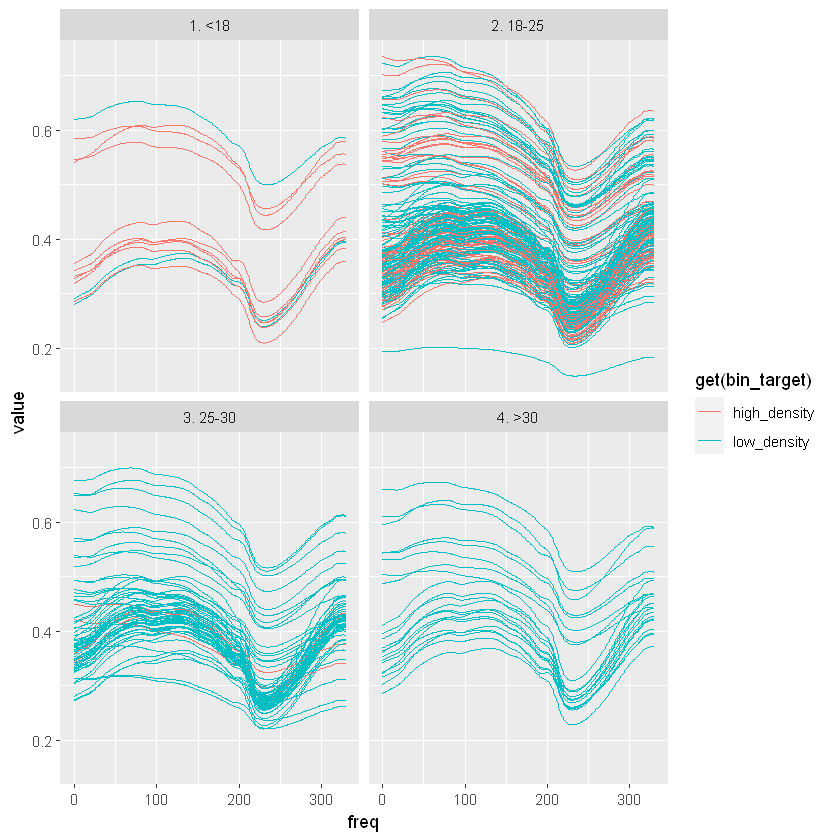
\includegraphics[trim={0 0cm 0cm 0}, clip, scale=0.55]{figures/scio_by_bmi.png}
	\caption{Distribution of spectrum values (for index 0 to 330), by different BMI categories.} 
	\label{fig:scio_bmi}
\end{figure}

\begin{figure}[!htb]
	\centering
	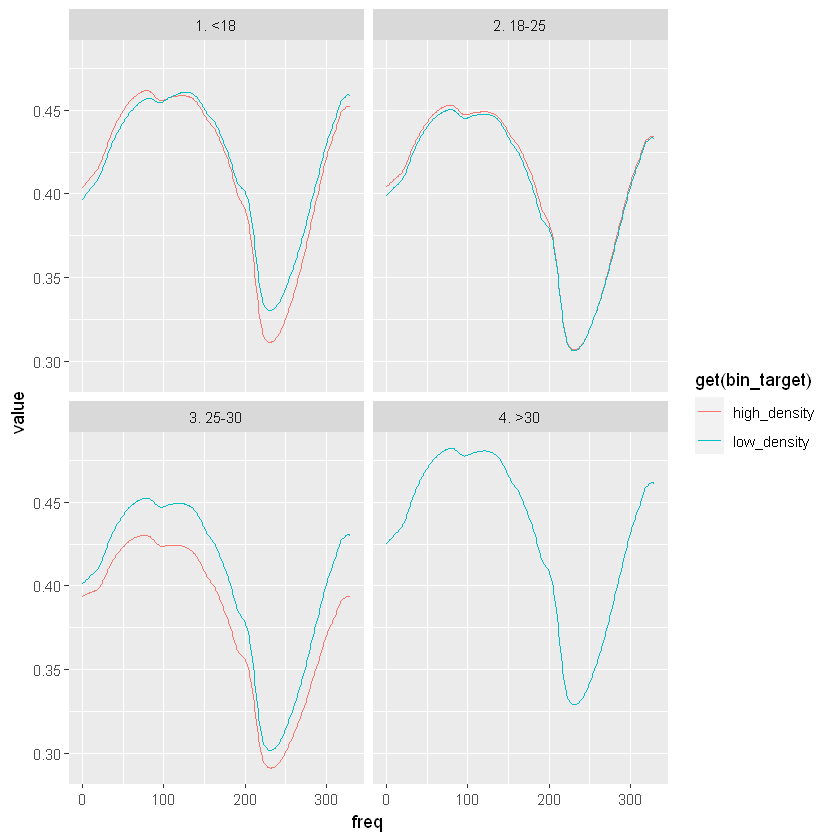
\includegraphics[trim={0 0cm 0cm 0}, clip, scale=0.55]{figures/scio_by_bmi_mean.png}
	\caption{Mean of spectrum values (for index 0 to 330), by different BMI categories.} 
	\label{fig:scio_bmi_mean}
\end{figure}

\begin{figure}[!htb]
	\centering
	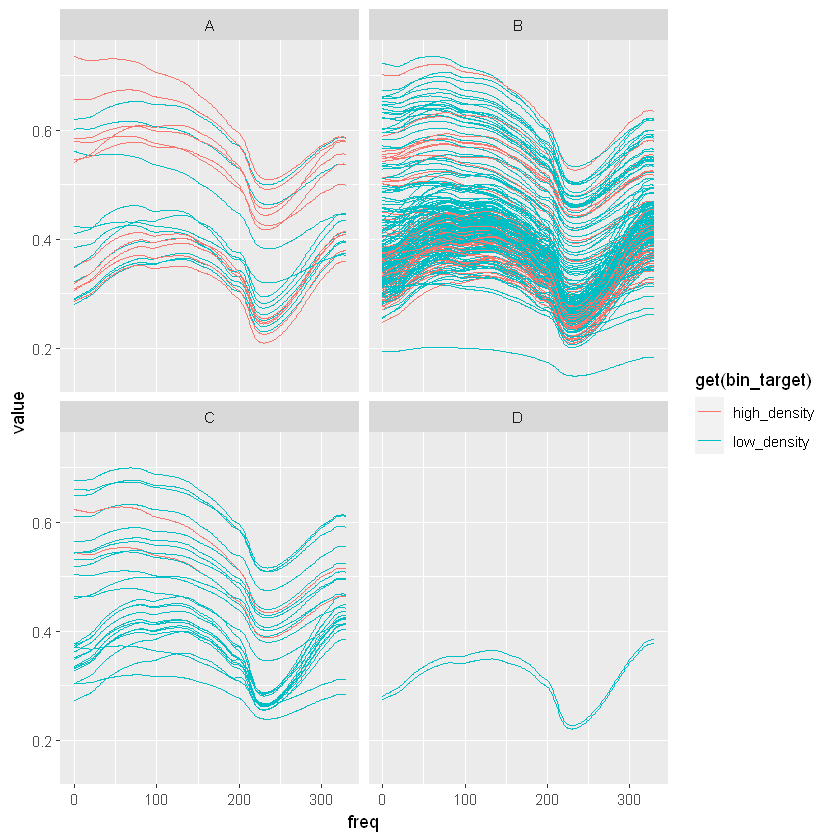
\includegraphics[trim={0 0cm 0cm 0}, clip, scale=0.55]{figures/scio_by_copa.png}
	\caption{Distribution of spectrum values (for index 0 to 330), by different BMI categories.} 
	\label{fig:scio_copa}
\end{figure}

\begin{figure}[!htb]
	\centering
	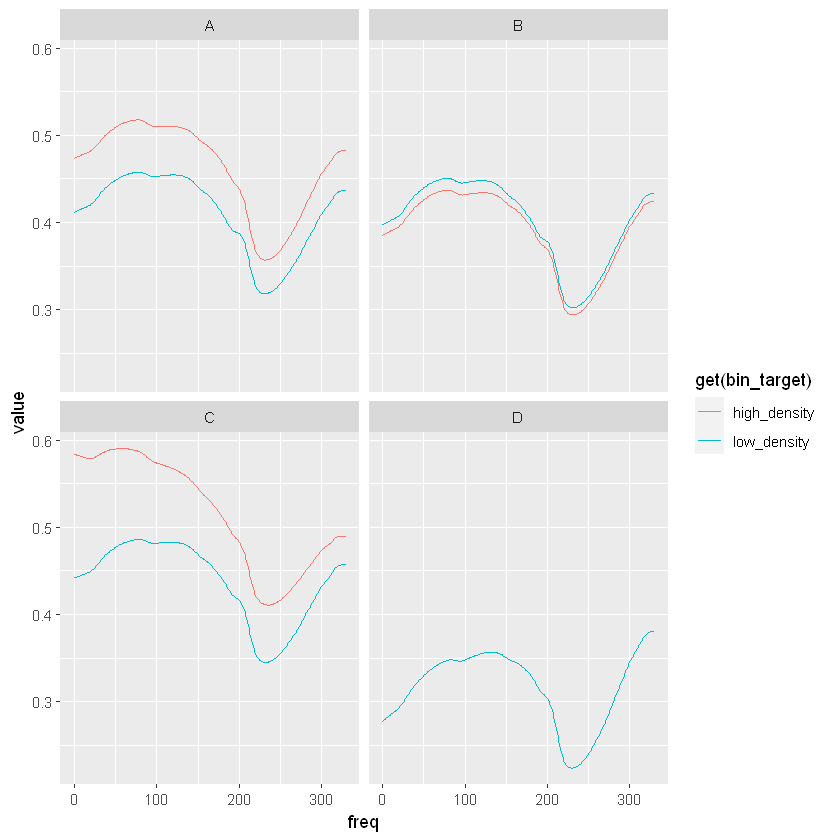
\includegraphics[trim={0 0cm 0cm 0}, clip, scale=0.55]{figures/scio_by_copa_mean.png}
	\caption{Mean of spectrum values (for index 0 to 330), by different BMI categories.} 
	\label{fig:scio_copa_mean}
\end{figure}

\begin{figure}[!htb]
	\centering
	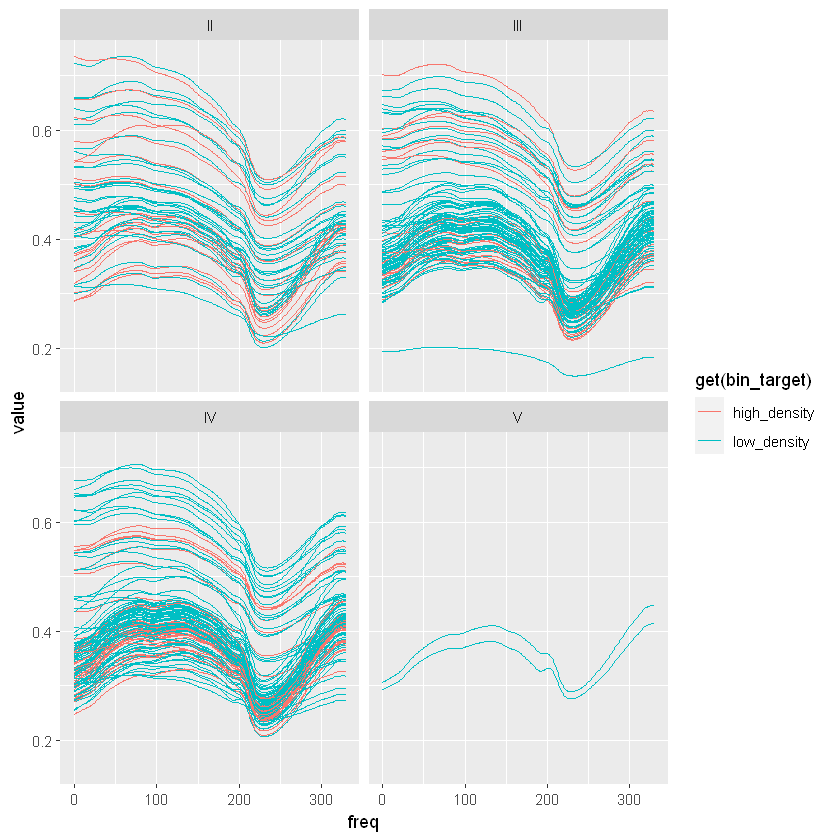
\includegraphics[trim={0 0cm 0cm 0}, clip, scale=0.55]{figures/scio_by_color.png}
	\caption{Distribution of spectrum values (for index 0 to 330), by different BMI categories.} 
	\label{fig:scio_color}
\end{figure}

\begin{figure}[!htb]
	\centering
	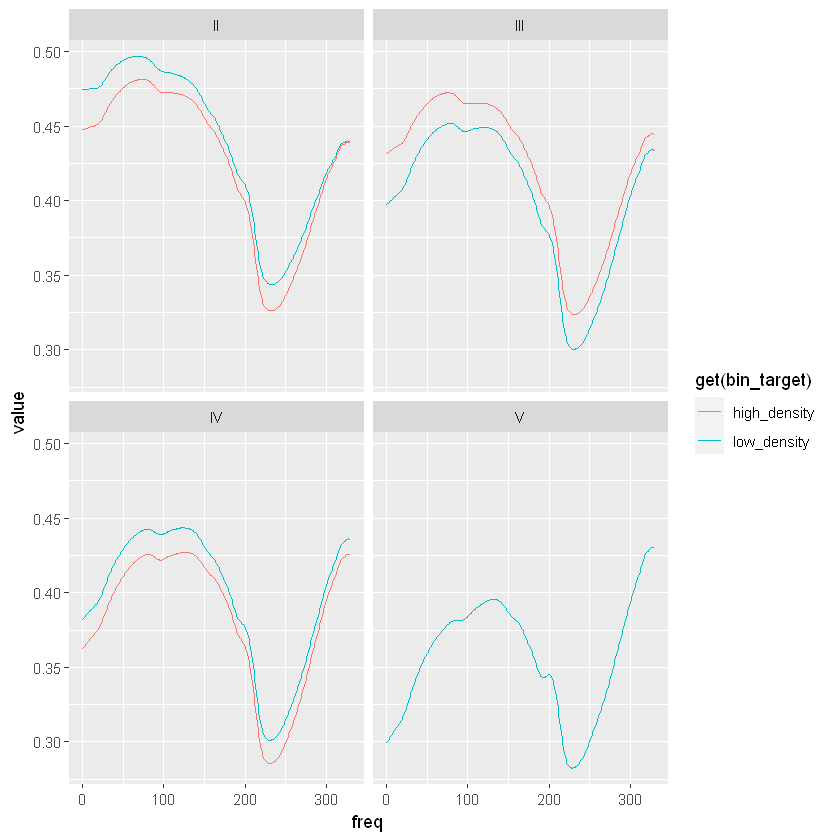
\includegraphics[trim={0 0cm 0cm 0}, clip, scale=0.55]{figures/scio_by_color_mean.png}
	\caption{Mean of spectrum values (for index 0 to 330), by different BMI categories.} 
	\label{fig:scio_color_mean}
\end{figure}

We conclude from this preliminary analysis that the spectrum variables, when controlling for some of these categorical features, can slightly differentiate high from low density individuals.

Another fact to highlight is the autocorrelation of the spectrum series. Figure \ref{fig:spectrum_ac} shows the average correlation an spectrum column (from 0 to 330) has with the $k-$the previous spectrums, for $k$ from 1 to 25. We see that these values are high (from almost 1 with $k=1$, an above $0.85$ for $k=25$. This suggest that looking at all columns of the spectrum in the analysis is redundant.

\begin{figure}[!htb]
	\centering
	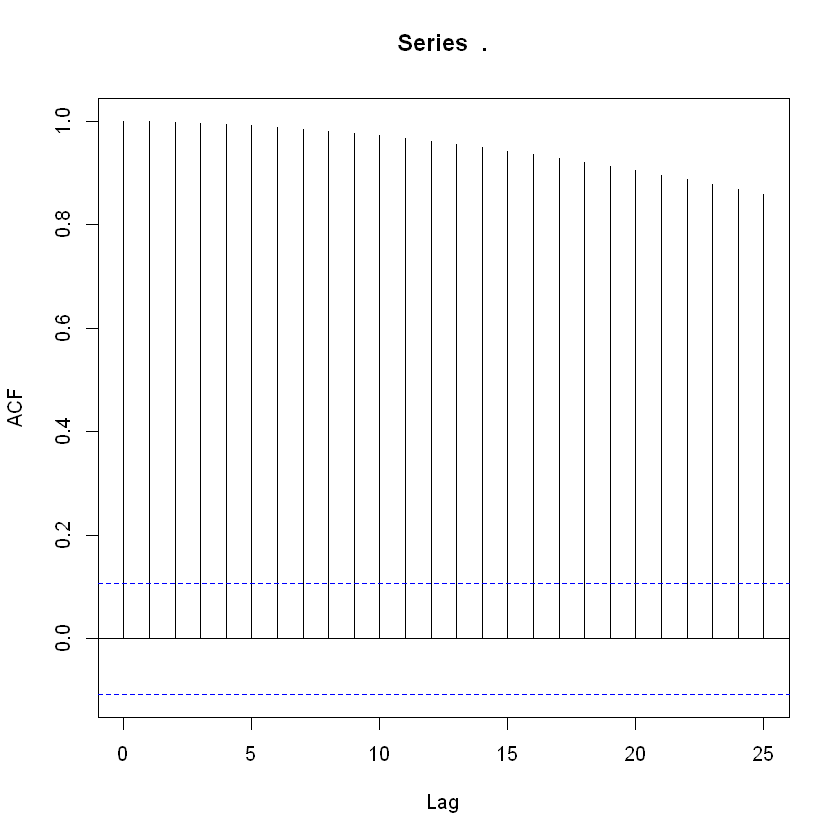
\includegraphics[trim={0 0cm 0cm 0}, clip, scale=0.55]{figures/spectrum_ac.png}
	\caption{Autocorrelation of spectrum values.} 
	\label{fig:spectrum_ac}
\end{figure}


\section*{Prediction}
Now we show the results of our classification prediction experiments. We consider as features the numeric BMI, age, Fitzpatrick color, and bra size. To aggregate spectrum, we took moving averages of size 50 and overlap of 25. This decision is taken based on the autocorrelation analysis, but the values of the window and overlap is somewhat arbitrary. As a target we considered the binary variable of high or low density, set at whether the DXA density is at value above or below 60 (which is roughly the 75\% quantile in the sample).

We built predictors using four different methods: logistic classification, support vector machine classifier, random forests, and optimal trees with hyperplanes. We compared the accuracy of our model -- and AUC, when available -- with that of the naive benchmark (predict largest category) and the model that does not consider spectrum as a feature. 

\begin{figure}[!htb]
	\centering
	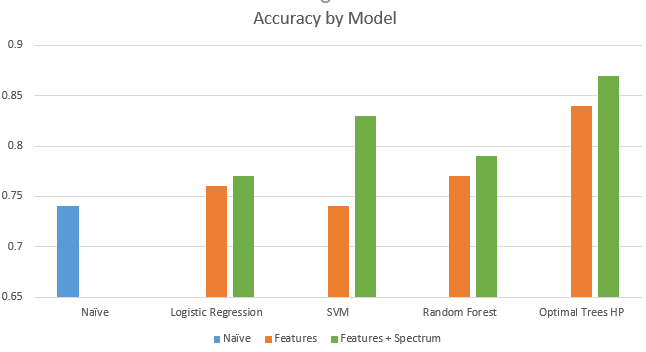
\includegraphics[trim={0 0cm 0cm 0}, clip, scale=0.55]{figures/accuracy_model.png}
	\caption{Accuracy of each model on test data (out of sample accuracy).} 
	\label{fig:accuracy_model}
\end{figure}

\begin{figure}[!htb]
	\centering
	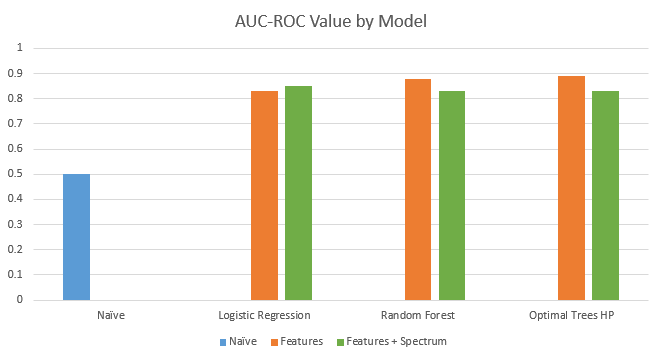
\includegraphics[trim={0 0cm 0cm 0}, clip, scale=0.55]{figures/auc_model.png}
	\caption{Accuracy of each model on test data (out of sample accuracy).} 
	\label{fig:auc_model}
\end{figure}

Both models outperform significantly the naive model. There exists some win in accuracy adding the spectrum values to the model, although it is not that significant. However, the difference grows slightly more than what is shown in the graph the smaller the moving average window becomes.

Next, we show the confusion matrix for each of this models. We compute the number of correct and incorrect label predicted for each class

\begin{table}[!htb]
	\centering
	\begin{tabular}{l|ll}
		Predicted/Actual & Low Density & High Density \\ \hline
		Low Density      & 66          & 24           \\
		High Density     & 4           & 28          
	\end{tabular}
	\caption{Logistic classification confusion matrix.}
\end{table}

\begin{table}[!htb]
	\centering
	\begin{tabular}{l|ll}
		Predicted/Actual & Low Density & High Density \\ \hline
		Low Density      & 72          & 18           \\
		High Density     & 3           & 29          
	\end{tabular}
	\caption{SVM confusion matrix.}
\end{table}

\begin{table}[!htb]
	\centering
	\begin{tabular}{l|ll}
		Predicted/Actual & Low Density & High Density \\ \hline
		Low Density      & 65         & 25           \\
		High Density     & 3           & 29          
	\end{tabular}
	\caption{Random Forest confusion matrix.}
\end{table}

\begin{table}[!htb]
	\centering
	\begin{tabular}{l|ll}
		Predicted/Actual & Low Density & High Density \\ \hline
		Low Density      & 82         & 8           \\
		High Density     & 4           & 24          
	\end{tabular}
	\caption{Optimal Tress with HP confusion matrix.}
\end{table}

Finally, we give an analysis based on the feature importance to show that although the spectrum is not the most relevant set of features, they are not negligible. TODO


\end{document}

